The result section will usually be tabulated or graphed, and each table or figure should be described, noting any interesting features – whether expected or unexpected, and in particular, inferences should relate to the original aims and objectives of the research outlined in the introduction. Results should be discussed and analysed, not simply presented blandly. Comparisons should also be drawn with the results or similar existing studies if relevant – do your results confirm or contradict those of previous research? Each table or figure should be mentioned explicitly in the text. Do not include in the project any tables or figures which are not discussed in the text. It is also worth trying to present the results in as interesting and varied way as possible – for example, including figures and charts as well as just tables.

\textbf{DUMMY TEXT}
The in-sample and out-of-sample forecasting ability of the different linear and nonlinear models described above were assessed in terms of statistical accuracy and economic criteria. The analysis was based on one-step-ahead forecasting. Once each model had been estimated, we constructed the in-sample and out-of-sample forecasts without updating the parameters of the model that were
obtained from the training set.

\chapter{Results}

Main points:

Få inn 
\begin{itemize}
    \item Graph 6.1: Vi ser en sammenehng mellom IV prosent og forecasting error. Det er altså vanskeligere å nøyaktig i størrelsesorden forutse høy IV-aksjer sin return. Dette er en pooled regression
    \item Vi bommer også mer på retning på høy IV stocks
    \item Men når vi treffer riktig retning, så er det på de store utslagene - som gjør at vi genererer positive alphaer, der alpha er definert som....
    \item Høy korrelasjon mellom IV og volatilitet 
    \item Ec. volatilitet har en høyere forklaringevne på alpha return enn bare IV isolert - det betyr at den systematiske risikoen som gjør at man kan forklare alpha.
\end{itemize}

\textbf{Table med regressjonsresultater - Alpha, beta, t-verdier, r sq.}

Table I shows the results of the goodness of forecasts for the different models and time periods and
for the corresponding forecast horizons. The main conclusions are two.

\begin{figure}[h]
    \centering
    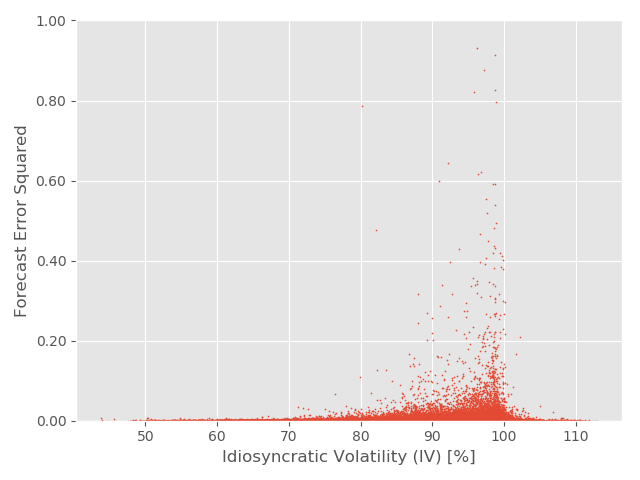
\includegraphics[scale = 1]{Plot/ScatterRegression.png}
    \caption{Regression: IV to forecasting error}
    \label{visualization}
\end{figure}

\begin{figure}[h]
    \centering
    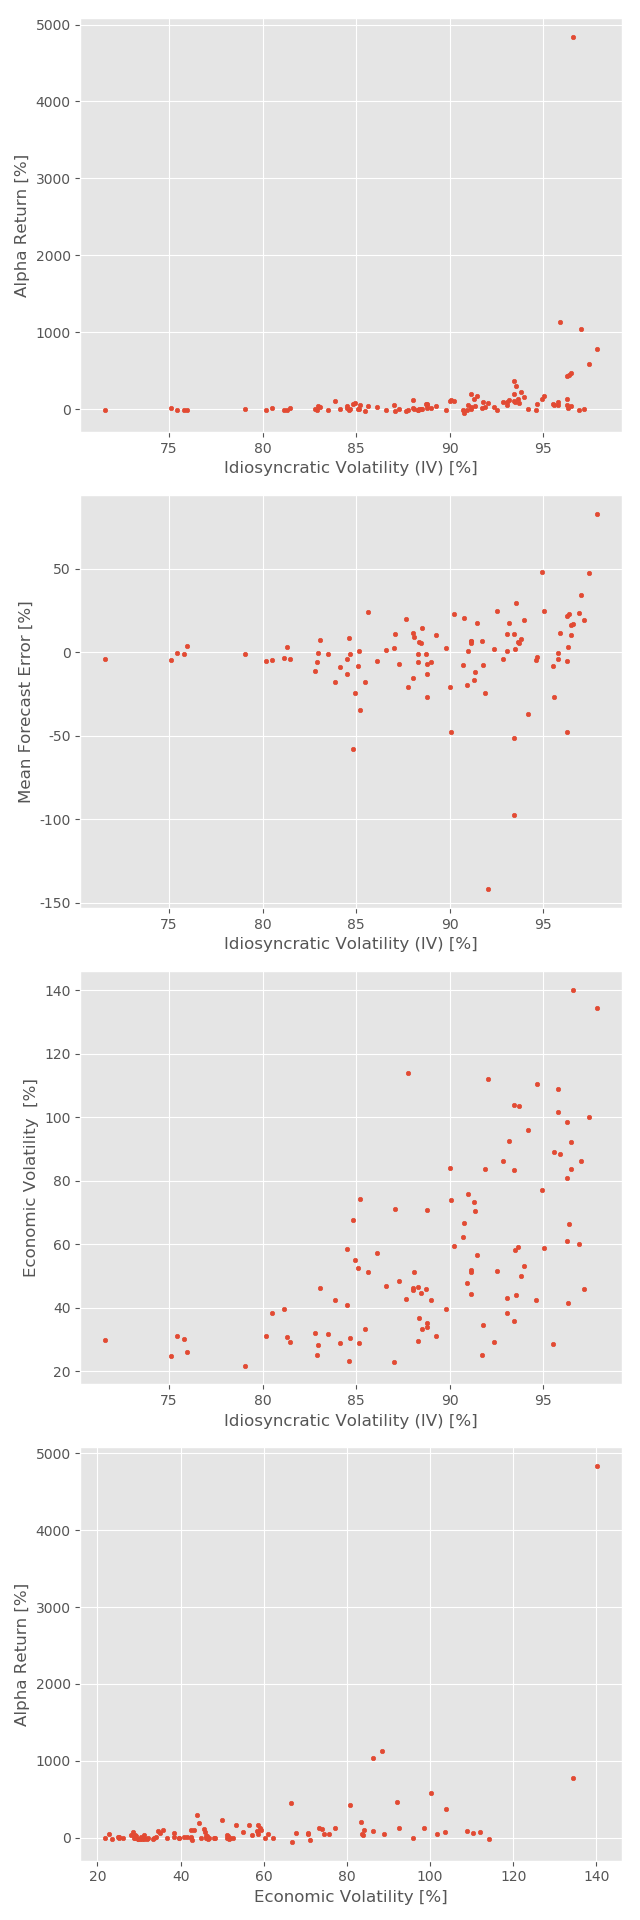
\includegraphics[height = 9 in , width = 5 in]{Plot/IndividualStockRegression.png}
    \caption{Regression: IV to forecasting error}
    \label{visualization}
\end{figure}






\newpage
\newcolumntype{P}[1]{>{\centering\arraybackslash}p{#1}}
\begin{landscape}
\begin{longtable}{P{1.5cm}P{1.5cm}P{1.5cm}P{1.5cm}P{1.6cm}P{1.5cm}P{1.5cm}P{1.5cm}P{1.5cm}P{1.5cm}P{1.5cm}P{1.5cm}} 
\caption{Forecast Stocks}
\label{Forecast Stocks}\\
\hline
\textbf{Bucket} & \textbf{IV }$\boldsymbol{\%}$ & $\boldsymbol{r_{economic}}$ & $\boldsymbol{\sigma_{economic}}$ & \textbf{Sign Ratio} &  $\boldsymbol{r_{sign}}$ & $\boldsymbol{\sigma_{sign}}$ & $\boldsymbol{\alpha}$ & $\boldsymbol{\bar\epsilon_{forecast}}$ & $\boldsymbol{\sigma_{forecast}}$ & $\boldsymbol{S_{economic}} $ & $\boldsymbol{S_{sign}}$ \\
\hline
\endfirsthead
\multicolumn{12}{c}%
{\tablename\ \thetable\ -- \textit{Continued from previous page}} \\
\hline
\textbf{Bucket} & \textbf{IV }$\boldsymbol{\%}$ & $\boldsymbol{r_{economic}}$ & $\boldsymbol{\sigma_{economic}}$ & \textbf{Sign Ratio} &  $\boldsymbol{r_{sign}}$ & $\boldsymbol{\sigma_{sign}}$ & $\boldsymbol{\alpha}$ & $\boldsymbol{\bar\epsilon_{forecast}}$ & $\boldsymbol{\sigma_{forecast}}$ & $\boldsymbol{S_{economic}} $ & $\boldsymbol{S_{sign}}$ \\
\hline
\endhead
\hline \multicolumn{12}{r}{\textit{Continued on next page}} \\
\endfoot
\hline
\endlastfoot
\input{Input/BucketTable.txt}
\end{longtable}
\end{landscape}



